\documentclass{article}
\usepackage{graphicx} % Required for inserting images
\usepackage{float}
\usepackage[T1]{fontenc}
\usepackage{amsmath}
\usepackage[margin=1in]{geometry}
\usepackage{booktabs}
\usepackage{tabularx}
\usepackage[hidelinks]{hyperref}

\title{Short-only book vs the live rule: R2 option backtest}
\author{Experiment report \textperiodcentered{} L/S Gamma Desk, QUANTT}
\date{2026-10-16}

\begin{document}

\maketitle

\textbf{Question:} Does turning long gamma off (short-only) give higher net P\&L than the live rule after costs, without a worse tail?

\textbf{Method:} One variant, \texttt{short\_\allowbreak{}only}, sets \texttt{[signal] long\_\allowbreak{}band = -\allowbreak{}inf} so the long signal never fires; everything else is the live \texttt{paper.\allowbreak{}toml}. It was replayed with the live code on R2 option trades (snapshots v1, config hash b040760187f0) over the development window 2014-06-02 to 2024-12-31, at 1x and 2x modelled spreads, with costs of \$0.65 per contract, \$0.005 per share and a \$1 minimum per order. It is compared with baseline trial 1 (the live rule) at the same spread multiple, against the pass bar pre-registered on the hypothesis card (commit 8d1f0fe) before any run. The hold-out (2025-01-01 to 2026-07-10) was not used. This report was written by Claude at the PM's request.

\section{Result vs the pass bar}

All three bars hold at both multiples, so the experiment \textbf{passes}. But the short-only book still loses money: \ensuremath{-}\$774 at 1x and \ensuremath{-}\$2,351 at 2x. It loses less than the live rule, which is what the bar asks for. It is not a profitable book.

\begin{center}\small
\begin{tabularx}{\linewidth}{>{\raggedright\arraybackslash}X >{\raggedright\arraybackslash}X l >{\raggedright\arraybackslash}X l}
\toprule
\textbf{Bar} & \textbf{1x: short\_only vs baseline} & \textbf{1x} & \textbf{2x: short\_only vs baseline} & \textbf{2x} \\
\midrule
1a. Net P\&L, full window & \ensuremath{-}\$774 vs \ensuremath{-}\$2,060 & pass & \ensuremath{-}\$2,351 vs \ensuremath{-}\$4,122 & pass \\
1b. Net P\&L, 2014-06..2019-12 & \ensuremath{-}\$875 vs \ensuremath{-}\$986 & pass & \ensuremath{-}\$1,261 vs \ensuremath{-}\$1,511 & pass \\
1c. Net P\&L, 2020-01..2024-12 & +\$101 vs \ensuremath{-}\$1,073 & pass & \ensuremath{-}\$1,090 vs \ensuremath{-}\$2,611 & pass \\
2. abs ES 5\% (daily) \ensuremath{\leq} 1.10 \ensuremath{\times} baseline & \$85.5 vs limit \$106.1 & pass & \$92.4 vs limit \$115.0 & pass \\
3. Max drawdown \ensuremath{\leq} 1.10 \ensuremath{\times} baseline & \$2,220 vs limit \$3,330 & pass & \$3,222 vs limit \$4,684 & pass \\
\bottomrule
\end{tabularx}
\end{center}

Other full-window numbers (not part of the bar):

\begin{center}\small
\begin{tabularx}{\linewidth}{>{\raggedright\arraybackslash}X l >{\raggedright\arraybackslash}X l >{\raggedright\arraybackslash}X}
\toprule
\textbf{} & \textbf{Baseline 1x} & \textbf{Short-only 1x} & \textbf{Baseline 2x} & \textbf{Short-only 2x} \\
\midrule
Sharpe (on \$250k paper capital) & \ensuremath{-}0.36 & \ensuremath{-}0.15 & \ensuremath{-}0.68 & \ensuremath{-}0.43 \\
Round trips & 131 & 100 & 131 & 100 \\
Win rate & 52\% & 57\% & 50\% & 54\% \\
Option commissions & \$262 & \$200 & \$262 & \$200 \\
Hedge commissions (orders) & \$914 (914) & \$770 (770) & \$914 (914) & \$770 (770) \\
\bottomrule
\end{tabularx}
\end{center}

\section{Charts}

\begin{figure}[H]\centering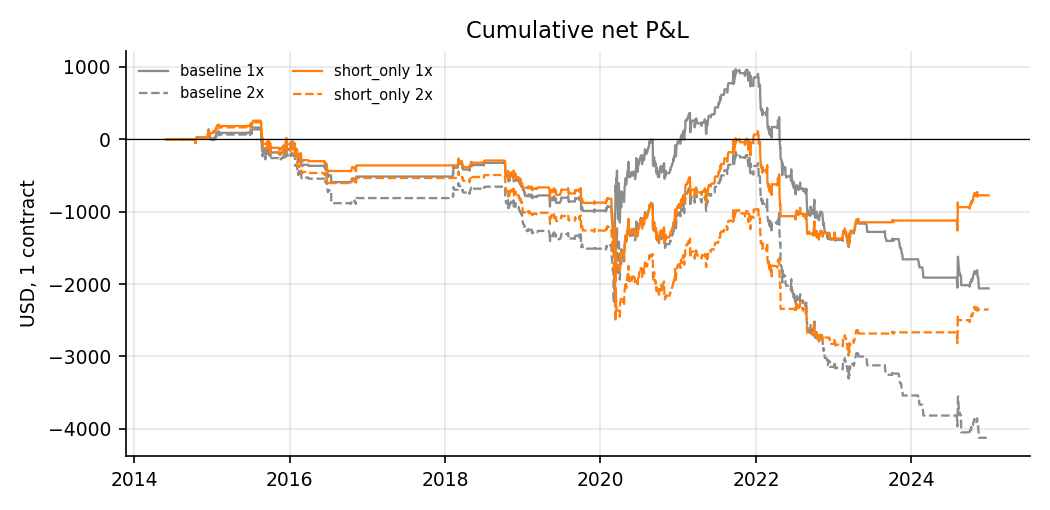
\includegraphics[width=0.92\linewidth]{figures/cum_pnl.png}\caption{Cumulative net P\&L, baseline (grey) and short-only (orange), solid 1x and dashed 2x.}\end{figure}

The two books track each other until 2020. After that the baseline does better through 2020--2021, then falls further from 2022. From 2023 the short-only book drifts up while the baseline keeps falling. At 1x the baseline is still about \$790 ahead at the end of 2021, so all of the final gap opens from 2022 on.

\begin{figure}[H]\centering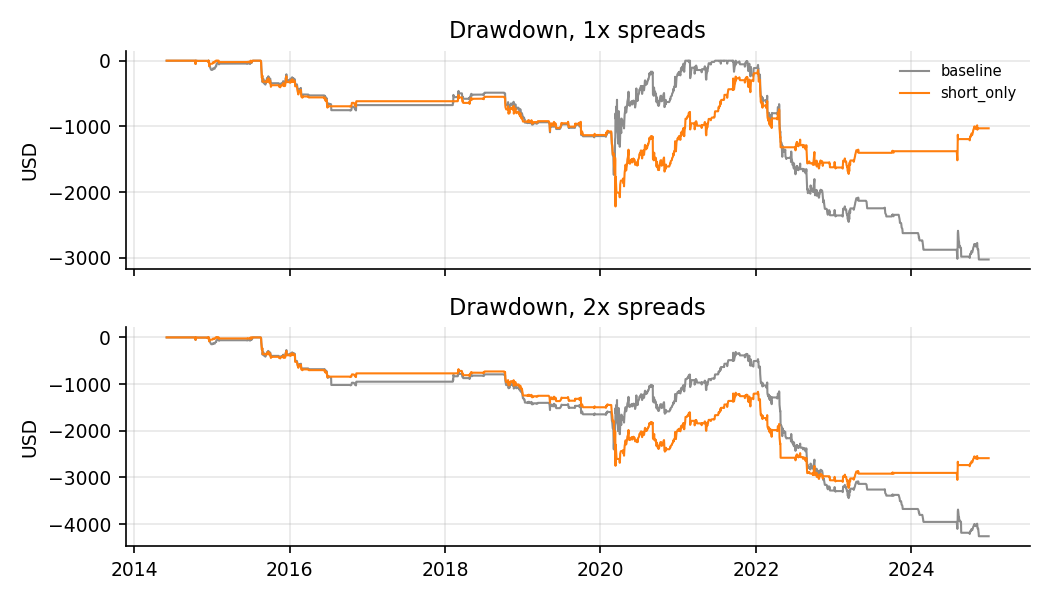
\includegraphics[width=0.92\linewidth]{figures/drawdown.png}\caption{Drawdown from the running peak at 1x and 2x spreads.}\end{figure}

The short-only book's deepest drawdown at 1x is the COVID crash (trough 2020-03-12), where it falls further than the baseline. The baseline's deepest drawdown is at the end of the window (trough 2024-11-14), after three losing years. At 2x the short-only trough is in March 2023.

\begin{figure}[H]\centering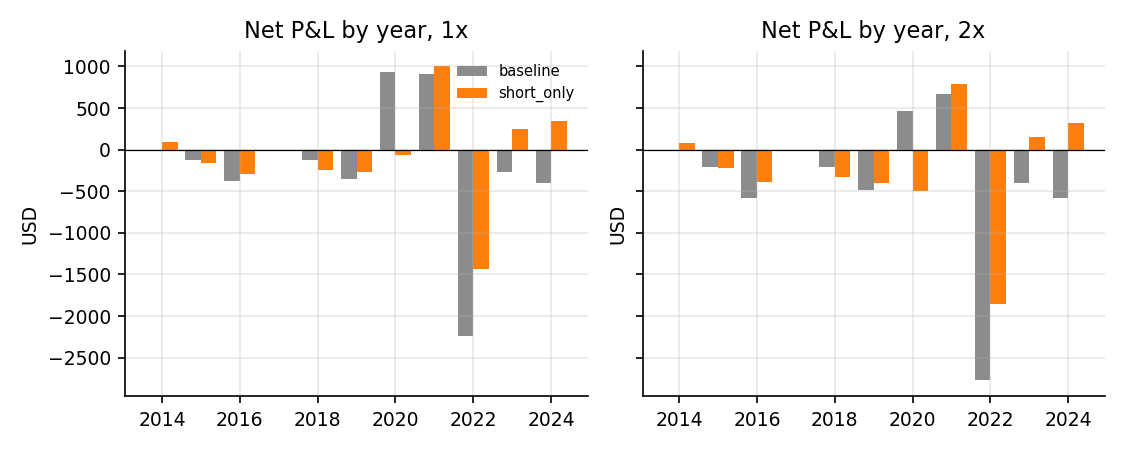
\includegraphics[width=0.92\linewidth]{figures/yearly.png}\caption{Net P\&L by calendar year at 1x and 2x.}\end{figure}

Short-only is better in 7 of 10 trading years at 1x (2017 had no signals). It is worse in 2015, 2018 and 2020. In 2020 the gap is about \$1,000, the year the baseline's flip exits protected its shorts. The biggest gains are 2022 (+\$809), 2023 (+\$517) and 2024 (+\$750), the years when the baseline's long trades lost most.

\begin{figure}[H]\centering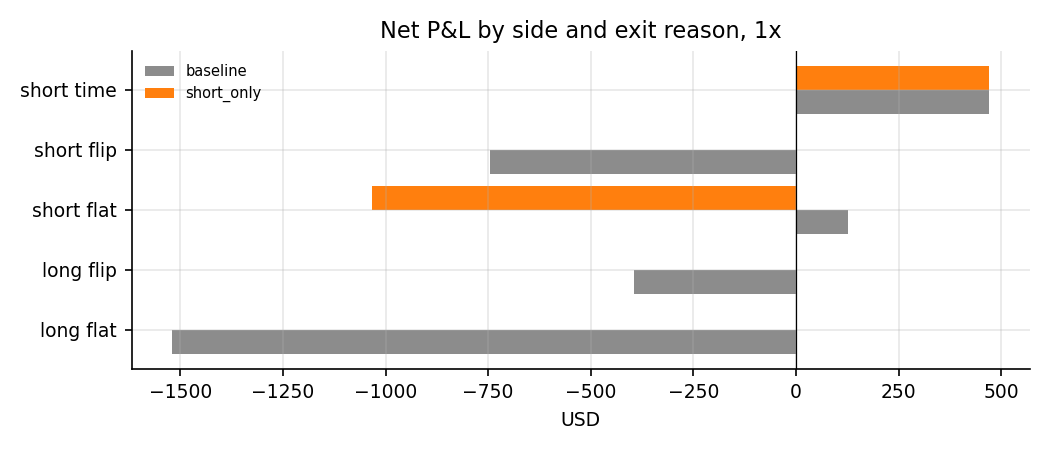
\includegraphics[width=0.92\linewidth]{figures/by_reason.png}\caption{Net P\&L of round trips by side and exit reason, 1x.}\end{figure}

Without a long signal, nothing closes a short by ``flip'' any more. The baseline closed 14 shorts on a long signal (\ensuremath{-}\$745 net at 1x). Short-only never opens one of them (entered 2020-03-12); the other 13 now wait for three flat days. That moves them into the ``flat'' bucket, which goes from +\$127 over 74 trades to \ensuremath{-}\$1,032 over 87 trades. Time exits are unchanged (13 trades, +\$470).

\begin{figure}[H]\centering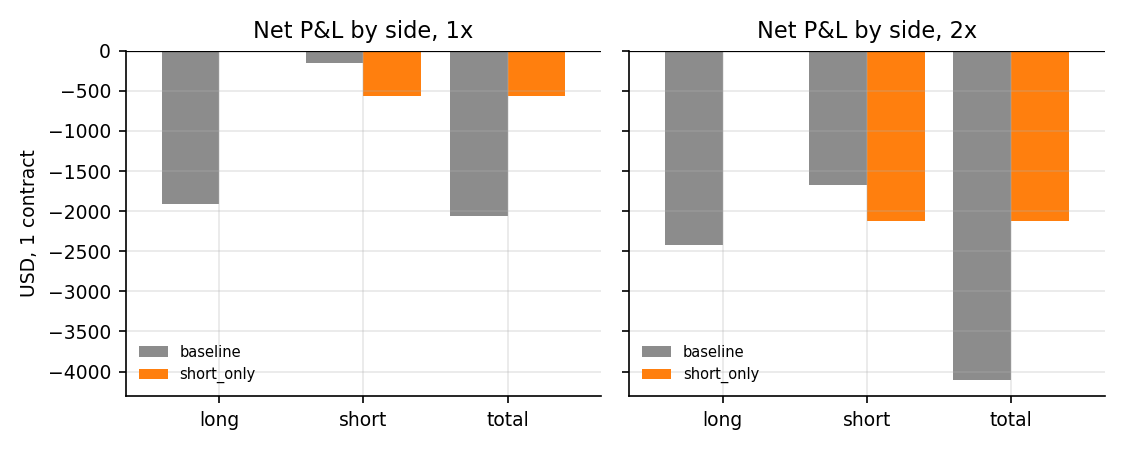
\includegraphics[width=0.92\linewidth]{figures/by_side.png}\caption{Net P\&L of round trips by side, baseline vs short-only, 1x and 2x.}\end{figure}

Dropping long removes the long side's \ensuremath{-}\$1,913 (1x) and \ensuremath{-}\$2,422 (2x) round-trip loss, but the short side gets worse: \ensuremath{-}\$562 vs \ensuremath{-}\$148 at 1x and \ensuremath{-}\$2,120 vs \ensuremath{-}\$1,679 at 2x. This chart sums round-trip net P\&L, but the pass bar uses daily equity. The two differ by the share unwind after each close (a \$1 minimum order plus the spot move between the decision snapshot and the fill). That residual is small for the baseline (+\$1 at 1x, \ensuremath{-}\$21 at 2x) and about \ensuremath{-}\$212 /\allowbreak{} \ensuremath{-}\$232 for short-only, so the ``total'' bars here don't match the table above exactly.

\begin{figure}[H]\centering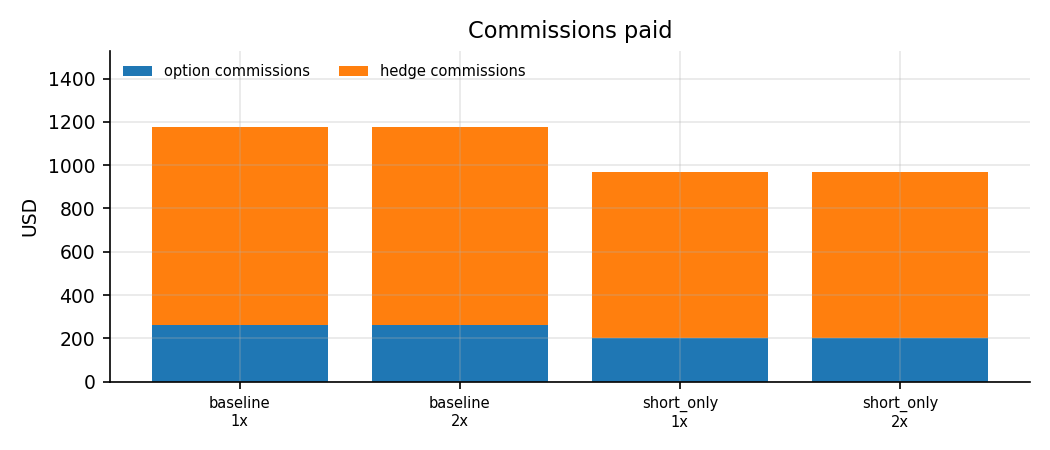
\includegraphics[width=0.92\linewidth]{figures/fees.png}\caption{Commissions paid, options and hedges.}\end{figure}

Short-only pays about \$206 less in commissions: 31 fewer option round trips and 144 fewer hedge orders. Hedge commissions are still about 80\% of the total, because of the \$1 minimum per order.

\section{Analysis}

The pass is driven by removing long trades, not by better shorts. The baseline's 30 long trades lost \$1,913 net at 1x, and long gamma lost money in every year except 2015, 2018 and 2021. Removing them improves the book by \$1,286 at 1x and \$1,771 at 2x. That is less than the long side's loss, because the shorts got worse.

The single position slot made no difference in this window. Every one of the 100 short-only shorts opened on a day the baseline also opened a short, and the baseline has one extra. So the books differ in two ways only: the long trades are gone, and short exits changed. In the baseline, a long signal (VRP below \ensuremath{-}5 pts, i.e. the RV forecast well above IV) closes an open short at once. That acted as an early stop: it got shorts out at the start of the March 2020 sell-off. In the short-only book those days count as flat, and the short waits three flat days, which cost about \$570 on 2020 shorts at 1x. So the long signal has value as an exit for shorts even though it has no value as an entry.

The margin is thin in the first half: \$111 at 1x and \$250 at 2x over 5.5 years, from 38--44 trades. The second half carries the result. There, short-only beats the baseline by \$1,175 at 1x and \$1,520 at 2x, mainly because it avoided the baseline's long losses in 2022--2024. The tail and drawdown bars pass comfortably, but short-only now holds its worst drawdown in a crash (2020) instead of a slow bleed. That is the profile a short-gamma book should expect.

\section{Verdict}

\textbf{Passed} at both 1x and 2x on all three pre-registered bars. On this window, the live long side destroys value after costs, and switching it off makes the book less negative without a worse tail. It does not make the book profitable: net P\&L is still \ensuremath{-}\$774 at 1x and \ensuremath{-}\$2,351 at 2x. The result is in-sample, because the idea came from the baseline on this same window, so it is not grounds to change \texttt{paper.\allowbreak{}toml}. Promotion needs the single hold-out run named on the card.

\section{Caveats}

\begin{itemize}

\item \textbf{In-sample idea.} The hypothesis came from the baseline's per-side split on this same window. A pass here is the expected outcome, not independent evidence. Only the hold-out run can confirm it.

\item \textbf{Size.} Everything is one contract, so the \$1 minimum per order is large relative to the position. Hedge commissions alone (\$770) are larger than the short-only book's gross round-trip P\&L at 1x (+\$318).

\item \textbf{Spread model.} The modelled half-spreads were fitted on about two weeks of calm 2026 live quotes. That is why the 2x run matters, and the bar passes at 2x too.

\item \textbf{Data gaps.} Month-end R2 days are missing (3.3\% of scheduled times skipped, the same in both books).

\item \textbf{Few events.} The first half has 38 short-only trades, and much of the second-half gain comes from three years. The 2020 result shows that removing the long signal also removes an exit that protected shorts in a crash.

\item \textbf{Attribution.} The side split (round trips) leaves out the share unwind after each close, so per-side numbers are approximate. The pass bar uses daily equity, which includes everything.

\end{itemize}

\section{Trials}

This comparison has four registered trials. There are 2 for \texttt{2026-\allowbreak{}10-\allowbreak{}16-\allowbreak{}short-\allowbreak{}only} (\texttt{short\_\allowbreak{}only} at 1x and 2x, one run, commit 8d1f0fe, clean). There are also 2 for \texttt{baseline} (trial 1 at 1x and 2x). The earlier baseline regression check that reproduced trial 1 was not registered. The experiment script was run once. Its reporting step crashed after both trials were registered: it read the registry while a parallel experiment was writing to it. Charts and tables were then rebuilt with \texttt{-\allowbreak{}-\allowbreak{}report-\allowbreak{}only}, which creates no trials.

\end{document}
